
		% Beobachten des Leakage-Effektes
		% nutzen der "Fenster"-Funktionen um Leakage-Effekt zu verminder (Signalverfälschung mit Hann-Fenster)
		% Schreiben einer Labview VI, die Amplitudenmodulation mit Hilfe der Sinus VI durchführt
		% falsche Verkabelung für Ausgabe des Signals über Soundkarte (Fehler zunächst nicht erkannt)
		% -> Verwendung des Funktionsgenerators für Modulation
		% Messstruktur um Demodulation für AM erweitern
		
		Zu Beginn des dritten Tages wurde die Arbeit an der Messstruktur fortgesetzt.
		Abb. \ref{fig:messstruktur} stellt das Endprodukt für diesen Aufgabenteil dar.
		
		\begin{figure}[H]
			\centering
			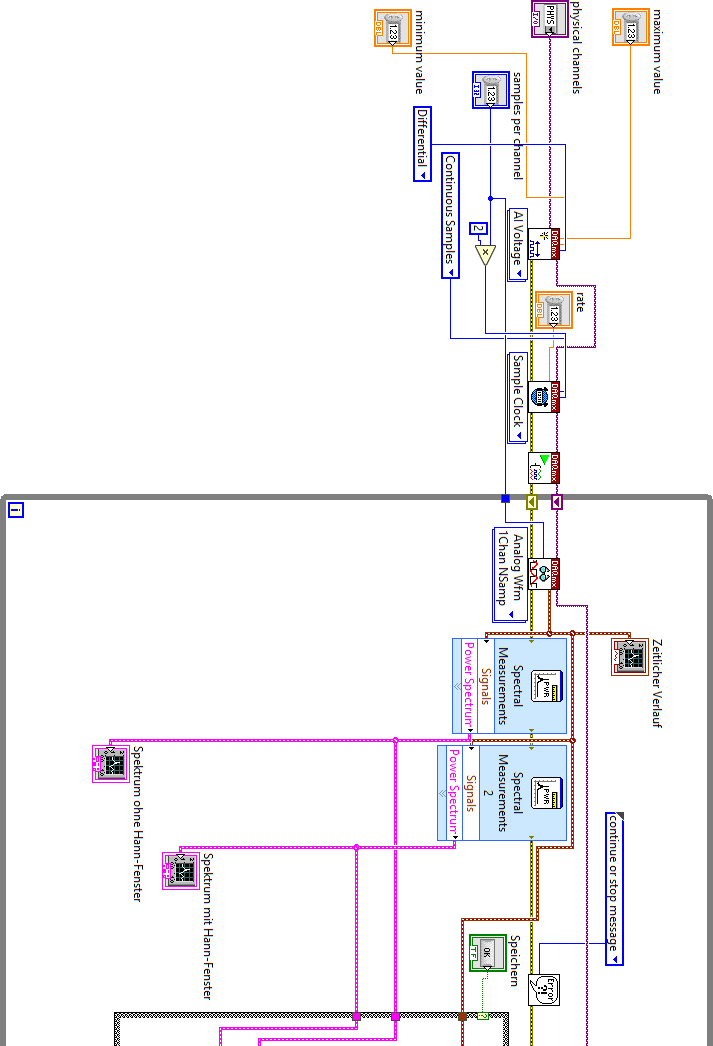
\includegraphics[width=\textwidth]{pic/messstruktur1.png}	
		\end{figure}
		
		\begin{figure}[H]
			\centering
			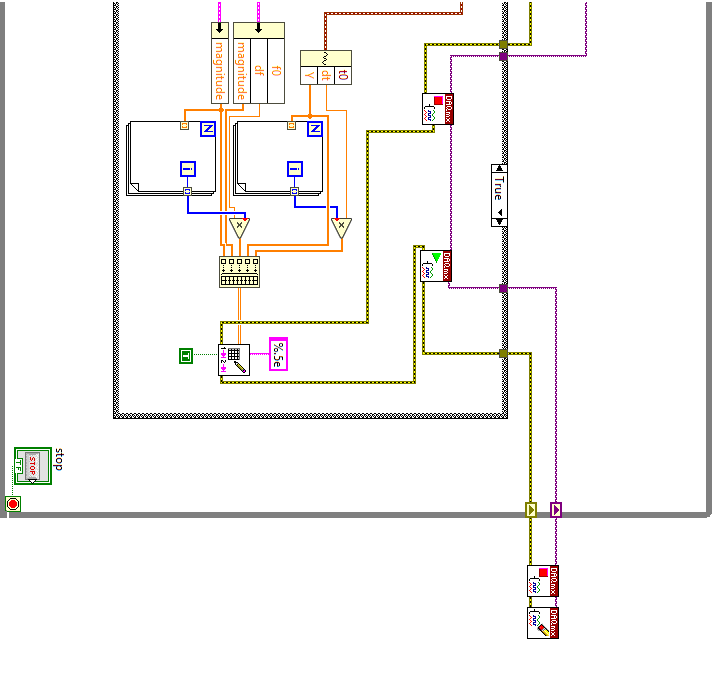
\includegraphics[width=\textwidth]{pic/messstruktur2.png}	
			\caption{text}
			\label{fig:messstruktur}
		\end{figure}
		
		\thispagestyle{plain}
		Ähnlich zu dem DAQ-Assistant sind hier die Eingänge für Anzahl der Datenpunkte und Messrate vertreten.
		Die VIs, welche die Funktionen des DAQ-Assistants ersetzen sollen sind die DAQmx-VIs, welche in Reihe geschaltet werden.
		Als Eingang in das erste DAQmx-VI wir der Kanal übergeben von dem das Signal empfangen werden soll, welcher hier "physical channel" heißt.
		Bei dem verwendeten Computer handelte es sich bei diesem Kanal um "Dev3/ai0".
		Da Spannungen im differentiellen Modus gemessen werden sollten wurden "AI Voltage" und "Differential" als Modus bzw. konstanter Eingang an das DAQmx-VI gelegt. 
		Um die gemessene Spannungen variabel zu begrenzen wurden zusätzlich Controls angebracht.
		Die Benennung dieser mit "minimum value" und "maximum value" entstammt der voreingestellten Namen der Eingänge des DAQmx-VIs.
		In einer späteren Version wurden die englischen Namen durch deutsche ersetzt.
		Von den Ausgängen dieses VIs gehen nur der Signalkanal und ein Fehlerkanal durch, welche sich von hier aus bis ans Ende der Messstruktur durch alle DAQmx-VIs ziehen.
		
		Das zweite DAQmx-VI dient als Taktgeber für die Aufnahme des Signals, deswegen der Modus "Sample Clock".
		Ihm werden einerseits der Signalkanal und der Fehler übergeben, andererseits auch die Messrate "rate" und die doppelte Anzahl der Datenpunkte "samples per channel", damit der CPU weniger ausgelastet wird. 
		Mit dem letzten und konstanten Eingang "Continuous Samples" wird festgelegt, wie die Daten aufgenommen werden.
		Da der Funktionsgenerator kontinuierlich ein Signal ausgibt, soll auch so lange getaktet werden, bis der Nutzer das Programm beendet.
		
		Das nächste DAQmx-VI ist nur für den Start des Messvorgangs zuständig.
		Von dort aus geht es in eine while-Schleife mit Stopp-Knopf, damit das Programm jederzeit von dem Benutzer beendet werden kann, ohne dass ein Stopp von Labview erzwungen werden muss.
		In dieser while-Schleife ist das erste Element ein weiteres DAQmx-VI.
		Dieses ist für das Lesen des Signals mit den vorgegebenen Parametern des Taktgebers verantwortlich.
		Es gibt ein dynamisches Array der Messdaten aus, welches mit Hilfe eines Waveform-Graphen auf der Frontplatte dargestellt werden kann.  
		Des Weiteren wird die Ausgabe für eine Spektralanalyse über zwei verschiedene Express-VIs genutzt. 
		Dabei wird bei einem mit dem sogenannten Hann-Fenster gearbeitet und bei dem anderen ohne.
		Das Hann-Fenster dient zur Manipulation der Messdaten, um die vorkommenden nicht ganzzahligen Frequenzen schärfer im Frequenzbild darzustellen, um den Leakage-Effekt zu unterdrücken, auf den später noch genauer eingegangen wird.
		
		Neben den Daten verläuft auch das Fehlerkabel durch die Express-VIs. 
		Falls ein Fehler in dem Programm auftritt dann wird aufgrund des VIs mit der Sprechblase eine Fehlermeldung ausgegeben und der Nutzer wird gefragt, ob das Programm weiterlaufen oder gestoppt werden soll.
		
		Um die ermittelten Daten für das Zeitbild und das Frequenzbild zu speichern wird die Case-Struktur nach der Spektralanalyse eingebaut.
		Wird auf den Speicherknopf auf dem Frontpanel gedrückt, so wird der in Abb. \ref{fig:messstruktur} dargestellte Fall durchgeführt.
		Andernfalls der in Abb. \ref{fig:messstruktur_case} dargestellte Fall, in dem das Programm einfach weiterläuft.
		\begin{figure}[H]
			\centering
			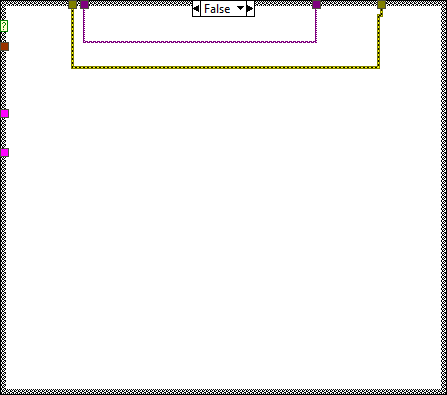
\includegraphics[width=0.5\textwidth]{pic/messstruktur_case.png}	
			\caption{text}
			\label{fig:messstruktur_case}
		\end{figure}
	
		Im Falle des Speicherns hingegen wird das Lesen der Daten über ein DAQmx-VI angehalten, damit überhaupt ein fester Datensatz gespeichert werden kann.
		Um die Daten zu erhalten werden das Signal des Zeitbildes und der Frequenzbilder in Waveform-Builder gegeben um die einzelnen Parameter zu erhalten.
		Damit die Zeit $t_i$ und die Frequenz $f_i$ dargestellt werden können, werden die Differentiale d$t$ und d$s$ über for-Schleifen $i$ mal aufaddiert.
		Aus diesen Zeiten und Frequenzen werden mit ihren jeweiligen Amplituden (\si{\volt} im Zeitbild und \si{\decibel} im Frequenzbild, mit und ohne Hann-fenster) in ein Array gegeben und in ein VI gegeben, welches eine Datei ausgibt, in dem das Array mit $i$ Zeilen und den fünf Spalten für die einzelnen Parametern ausgegeben wird.
		An diesem VI lässt sich auch das Format der Daten darstellen, hier wurde "\%.5e" gewählt für eine Ausgabe wie in Tab. \ref{tab:speichern} für die exponentielle Schreibweise und fünf Nachkommastellen.	
		\begin{table}[ht]
			\centering
			\begin{tabular}{S S S S S}
				
				\text{0,00000E+0} &	\text{0,00000E+0} &	\text{1,21707E+0} &	\text{-4,15539E+1} &	\text{-5,78080E+1}\\
				\text{1,00000E-3} &	\text{1,00000E+0} &	\text{-6,34577E-1} &	\text{-3,99954E+1} &	\text{-6,09291E+1} \\
				\text{2,00000E-3} &	\text{2,00000E+0} &	\text{-2,24044E+0} &	\text{-4,00174E+1} &	\text{-9,43314E+1} \\
				\text{3,00000E-3} &	\text{3,00000E+0} &	\text{-2,98161E+0} &	\text{-4,00395E+1} &	\text{-8,78620E+1} \\
				$\colon$ \\		
				$\colon$ \\		
			\end{tabular}
			\caption{Beispielausgabe nach Nutzung der Speicherfunktion der Messstruktur.}
			\label{tab:speichern}
		\end{table}
		Eine automatische Benennung der Spalten ist hierbei nicht möglich, weswegen verfolgt werden muss welcher Wert an welcher Stelle in das Array eingefügt wird.
		
		Danach wird die Schleife wiederholt bis sie durch Betätigen des Stopp-Knopfes verlassen wird.
		Nach zwei weiteren DAQmx-VIs wird das Programm dann beendet.
		
	\subsection{Abtastung mit der Messstruktur}
	
		